\section{Model Training}

\subsection{Model Architecture}

We present the overall framework of Grounding DINO 1.5 series in Figure~\ref{fig:gd1.5_framework}. This framework retains the dual-encoder-single-decoder structure of Grounding DINO and extends it into Grounding DINO 1.5 for both the Pro and Edge models, which are introduced in Sections~\ref{gd1.5_pro_introduction} and \ref{gd1.5_edge_introduction}, respectively.

\begin{figure}[ht!]
\centering
 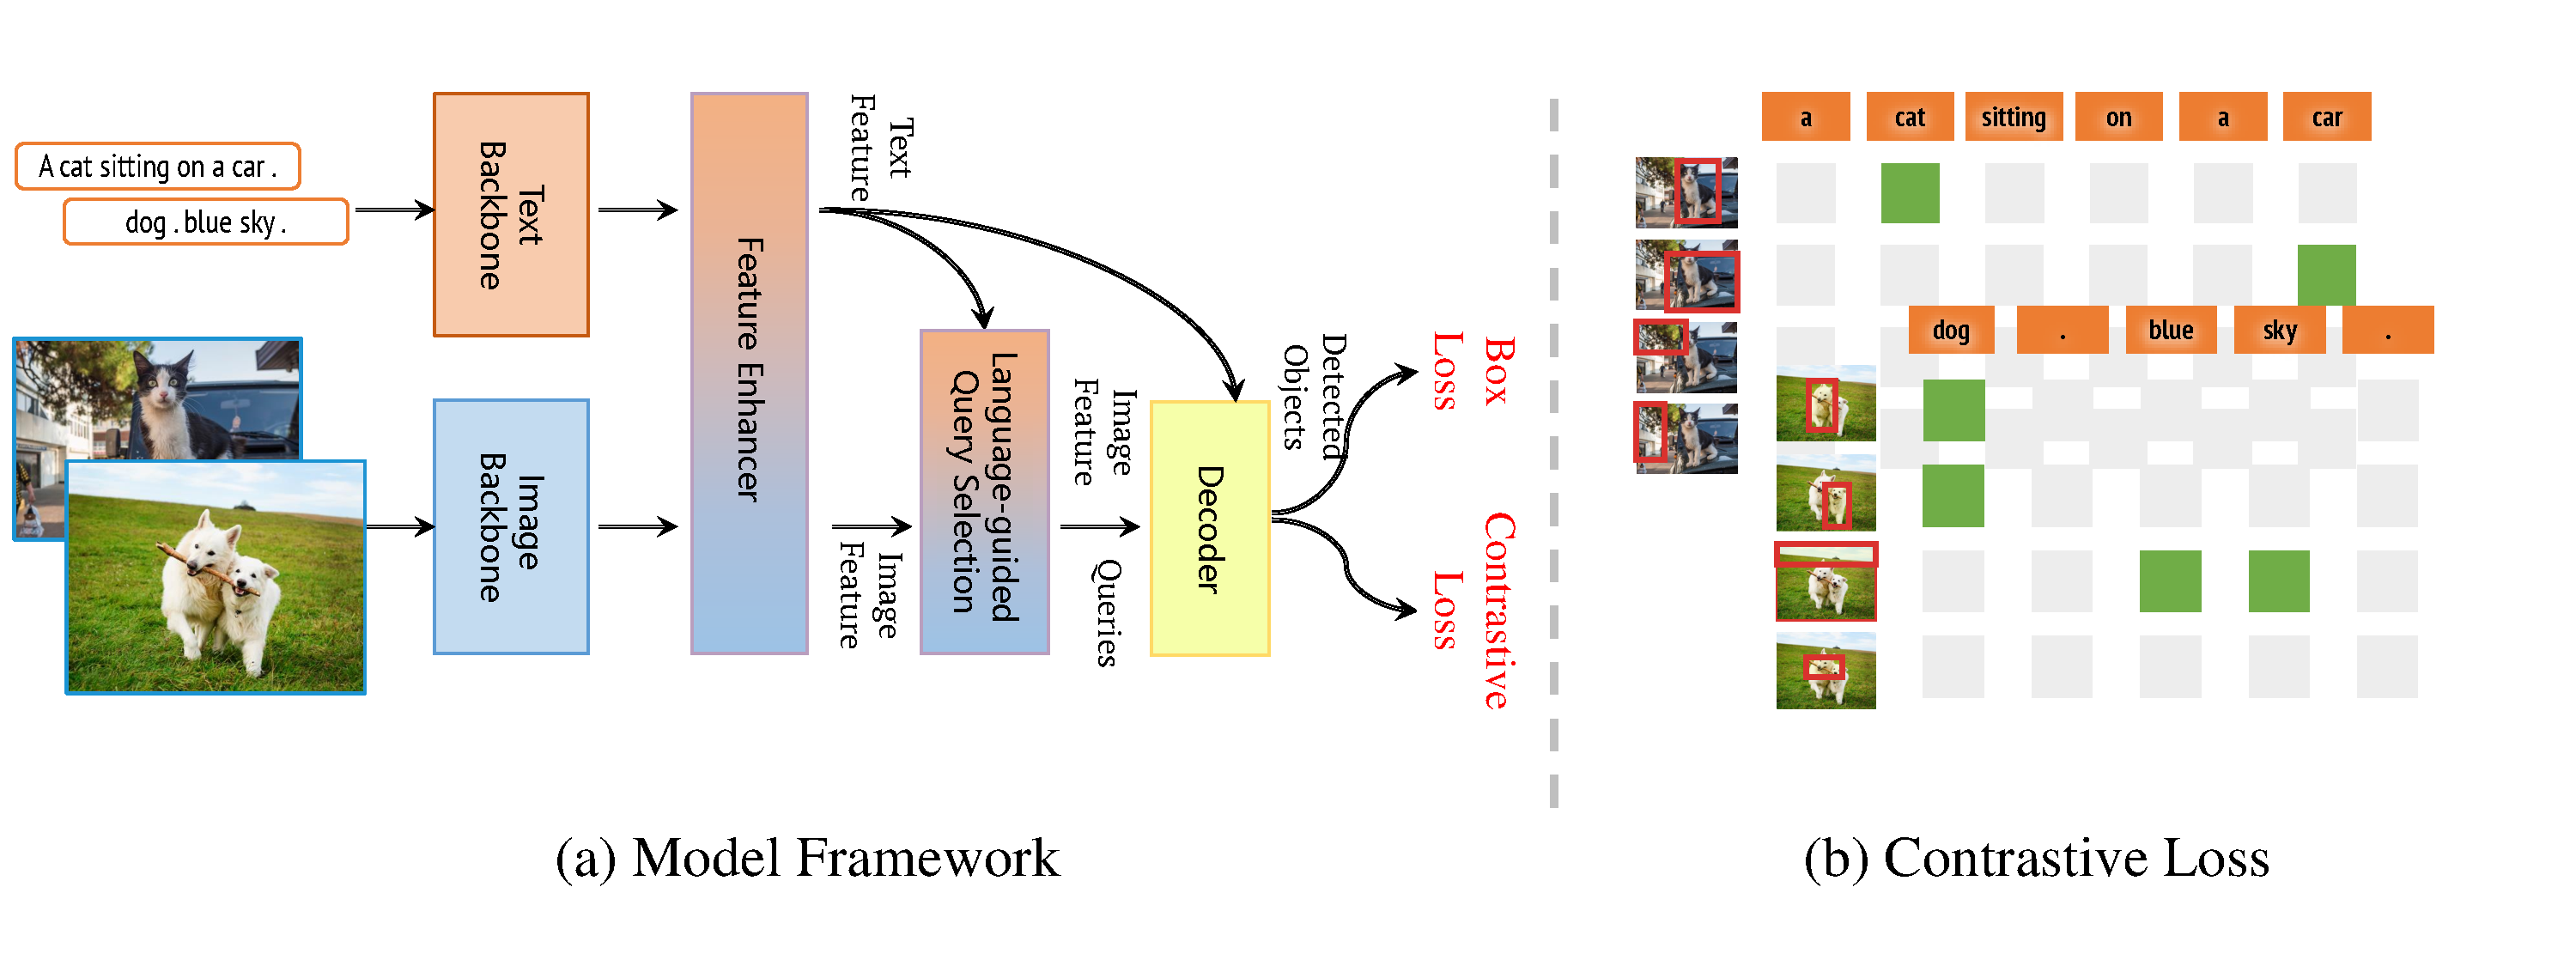
\includegraphics[width=1.0\textwidth,keepaspectratio]{figs/gd1.5_framework_v2.pdf}
 \caption{Grounding DINO 1.5 series overall framework.}
 \label{fig:gd1.5_framework}
\end{figure}

\subsubsection{Grounding DINO 1.5 Pro}
\label{gd1.5_pro_introduction}

Grounding DINO 1.5 Pro preserves the core architecture of Grounding DINO while incorporating a larger Vision Transformer backbone. We adopt the pre-trained ViT-L~\cite{EVA-02} model as our primary vision backbone for its superior performance on downstream tasks and its pure Transformer design, which lays a solid foundation for optimizing the training and inference processes.

% \paragraph{Discussions: early-fusion and late-fusion models.}
Following the methodologies of Grounding DINO~\cite{GroundingDINO} and GLIP~\cite{GLIP}, Grounding DINO 1.5 Pro employs a {deep early fusion} strategy during feature extraction. This involves cross-attention mechanisms between language and image features before the decoding phase, facilitating a more integrated information fusion.

We also compared the strategies of early fusion and later fusion. We observe that models trained with early fusion architecture design tend to yield a higher detection recall and better bounding box precision accuracy. However, this approach can also lead to increased model hallucinations, such as predicting objects not present in the input images.
In contrast to early fusion, the models with a late fusion design, which integrate language and image modalities only in the loss calculation phase, generally demonstrate robustness against hallucinations but may lead to lower detection recall. This is primarily due to the increased challenge of vision and language alignment as late fusion keeps features from different modalities separately until the loss phase. %However, this approach is less efficient in terms of modality alignment, which can adversely impact the predictive results of the model.

Consequently, to simultaneously enhance the model's prediction capability and maintain its robustness during inference, we have retained the early fusion design while introducing a more comprehensive training sampling strategy, which increases the proportion of negative samples during training. Such improvements facilitate achieving a balance between the advantages and drawbacks of the early fusion architecture.

\subsubsection{Grounding DINO 1.5 Edge}
\label{gd1.5_edge_introduction}

Deploying Grounding DINO on edge devices is highly desired by many applications, including autonomous driving, medical image processing, computational photography, etc. However, there is a large gap between the computational cost required by an open-set detection model and the limited resources available on edge devices. 
Grounding DINO uses multi-scale image features and a heavy computational feature enhancer for faster training and better performance, which is impractical for real-time scenarios in real-world applications.
% In Grounding DINO, to accelerate training convergence and improve performance, multi-scale image features are introduced, which results the feature enhancer module suffers from a high computational cost due to the deformable self-attention, it makes using Grounding DINO in real-world applications impractical. 

%In Grounding DINO, a feature enhancer which stacked by multi-layer feature enhancer layer, is proposed to fuse vanilla image features and vanilla text features. In each feature enhancer layer, two modal vanilla features are first enhanced by the deformable self-attention and the vanilla self-attention, then, feature fusion is achieved by cascading an image-to-text cross-attention with a text-to-image cross-attention. 

To overcome this obstacle, we propose a novel efficient feature enhancer, as shown in Fig.\ref{fig:efe}.
Recognizing that lower-level image features lack semantic information and introduce excessive computational costs, as demonstrated in Lite-DETR~\cite{LiteDETR}, we limit cross-modality fusion to high-level image features (P5 level) only. This approach greatly reduces the number of tokens that need to be processed, significantly cutting the computational demands of the feature enhancer. To facilitate easier deployment on edge-side GPUs, we replace deformable self-attention with vanilla self-attention, and introduce a cross-scale feature fusion module~\cite{zhao2023detrs} to integrate low-level image features (from P3 and P4 levels). Such a design effectively balances feature enhancement and computational efficiency.
% Recognizing that the interactions between text features and lower-level image features are unnecessary due to the lack of semantic concepts, we focus cross-modality fusion exclusively on high-level image features (P5), this strategy substantially reduces the computational cost of deformable self-attention by significantly decreasing the number of tokens processed. 
% To facilitate easier deployment on edge-side GPUs, we replace deformable self-attention with vanilla self-attention. Additionally, to compensate the detailed information lost from high-level image features, the cross-scale feature fusion module\cite{zhao2023detrs} is introduced to fuse lower-level image features(P3, P4). This allows for a balanced enhancement of feature representation while maintaining computational efficiency.

In our edge-optimized model, Grounding DINO 1.5 Edge, we replace the original feature enhancer with our newly proposed efficient one and employ EfficientViT-L1~\cite{Cai_2023_ICCV} as the image backbone for rapid multi-scale feature extraction. We deploy the model on the NVIDIA Orin NX platform, achieving an inference speed of over 10 FPS at an input size of 640 $\times$ 640. The visualization of the model predictions on NVIDIA Orin NX is shown in Figure~\ref{fig:edge_vis}, which demonstrates the effectiveness of our modifications in real-world edge computing environments.
% In our edge-optimized variant, Grounding DINO-Edge, we substitute the original feature enhancer with our newly efficient feature enhancer. Additionally, we use InceptionNeXt-T\cite{yu2023inceptionnext} as image backbone to extract multi-scale image features rapidly. This model is deployed on the Nvidia Orin NX platform, where it achieves an inference speed of 10 frames per second (FPS). The visualization on the Nvidia Orin NX is shown in \ref{fig:edge_vis}, illustrating the effectiveness of our modifications in real-world edge computing environments.

\begin{figure}[ht!]
\centering
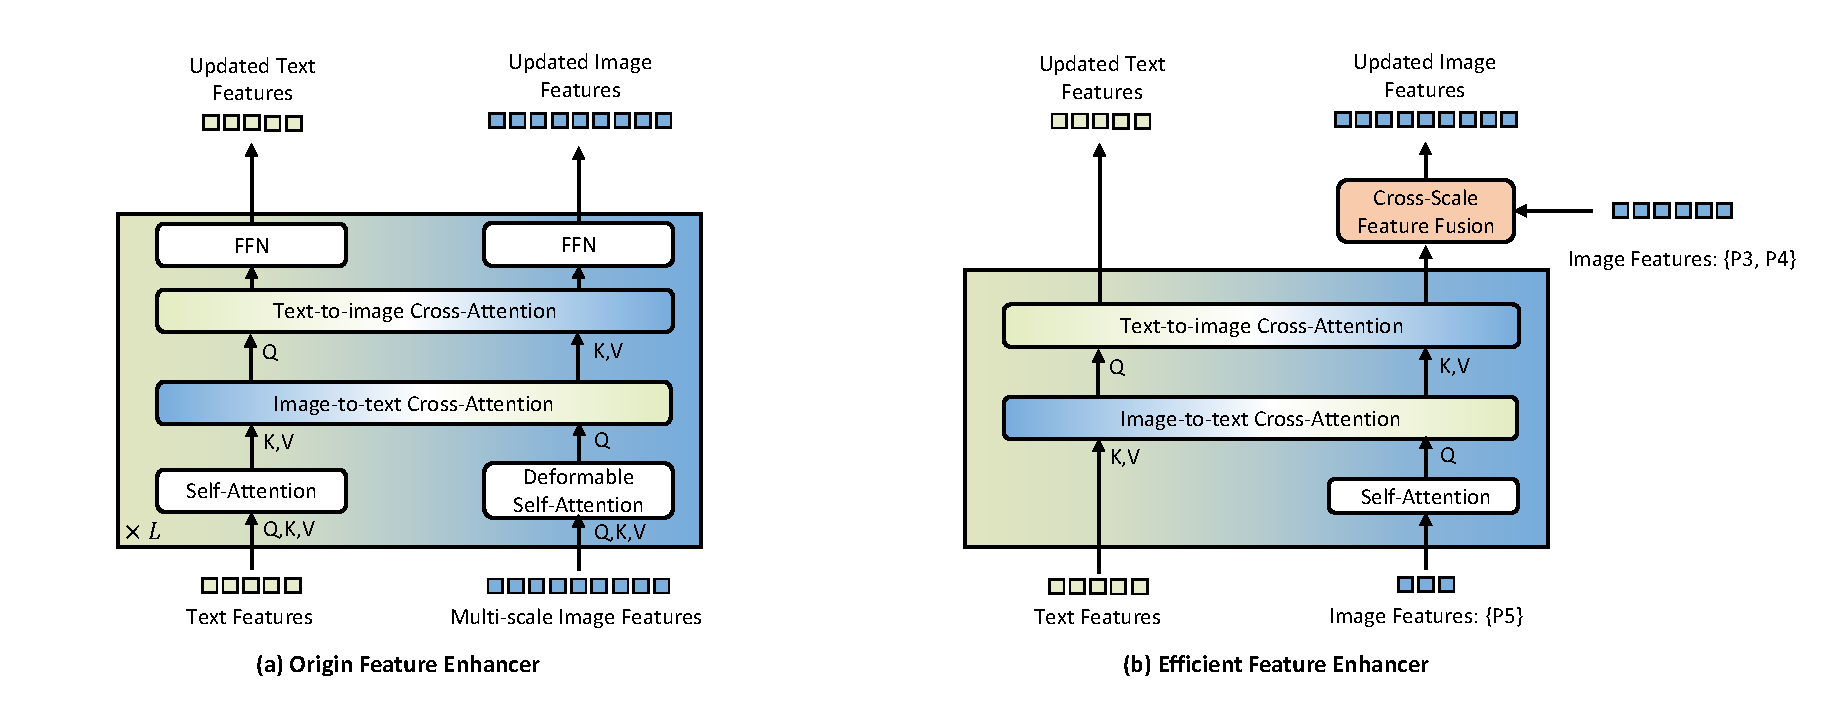
\includegraphics[width=0.95\textwidth,keepaspectratio]{figs/EFE.pdf}
\centering
\caption{Comparison of the Origin Feature Enhancer and the New Efficient Feature Enhancer.}
\label{fig:efe}
\end{figure}

\subsection{Training Dataset}
To train a robust open-set detector, it is crucial to construct a high-quality grounding dataset that is sufficiently rich in categories and encompasses a wide range of detection scenarios. Grounding DINO 1.5 is pre-trained on over 20M grounding images, termed \textbf{Grounding-20M}, which are collected from publicly available sources. We have carefully developed a series of annotation pipelines and post-processing rules to guarantee the high quality of the grounding annotations.

